\documentclass[tikz,border=5pt]{standalone}
% -- -- -- -- -- -- -- -- -- -- -- -- -- -- -- -- -- -- -- -- -- -- -- -- -- --
\begin{document}
% -- -- -- -- -- -- -- -- -- -- -- -- -- -- -- -- -- -- -- -- -- -- -- -- -- --
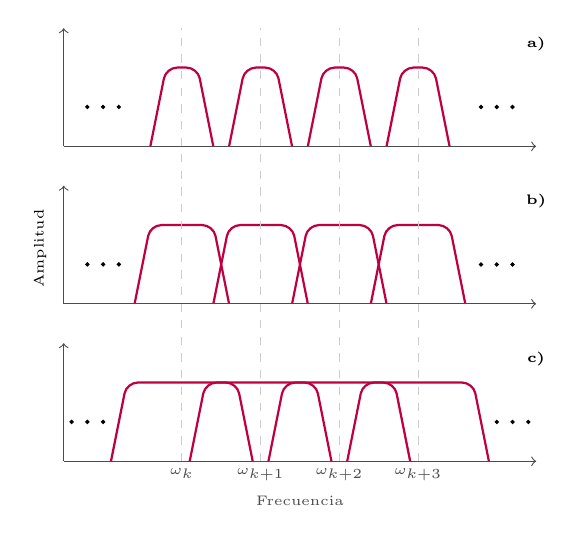
\begin{tikzpicture}
%				\draw[step=0.5,help lines] (0,-1) grid (8,6);
\tiny
% body of the graph
				\foreach \i in {1,2,3,4}
				\draw [purple, thick, rounded corners] (\i-0.4,0) -- (\i+0.2-0.4,1) --
				(\i+0.8+0.4,1) --	(\i+1+0.4,0);
				\foreach \i in {1,2,3,4}
				\draw [purple, thick, rounded corners] (\i-0.1,2) -- (\i+0.2-0.1,3) --
				(\i+0.8+0.1,3) --
				(\i+1+0.1,2);
				\foreach \i in {1,2,3,4}
				\draw [purple, thick, rounded corners] (\i+0.1,4) -- (\i+0.2+0.1,5) --
				(\i+0.8-0.1,5) --	(\i+1-0.1,4);
% draw axis
    \draw[->,black!70] (0,4) -- (0,5.5); 
    \draw[->,black!70] (0,2) -- (0,3.5); \draw(-0.3,2.7) node[rotate=90]
				{Amplitud};
    \draw[->,black!70] (0,0) -- (0,1.5);
    \draw[->,black!70] (0,0) -- (6,0);% node[below] {$\omega'$};
    \draw[->,black!70] (0,2) -- (6,2);% node[below] {$\omega'$};
    \draw[->,black!70] (0,4) -- (6,4);% node[below] {$\omega'$};
% draw axis label
    %\draw[black!70] (0.0,0) node[below] {$0$};
				\draw[black!70] (3,-0.5) node[] {Frecuencia};
				\draw[black!70] (1.5,0) node[below] {$\omega_{k}$};
				\draw[black!70] (2.5,0) node[below] {$\omega_{k+1}$};
				\draw[black!70] (3.5,0) node[below] {$\omega_{k+2}$};
				\draw[black!70] (4.5,0) node[below] {$\omega_{k+3}$};

				\draw [fill] (0.1,0.5) circle [radius=0.02];
				\draw [fill] (0.3,0.5) circle [radius=0.02];
				\draw [fill] (0.5,0.5) circle [radius=0.02];
				\draw [fill] (0.3,2.5) circle [radius=0.02];
				\draw [fill] (0.5,2.5) circle [radius=0.02];
				\draw [fill] (0.7,2.5) circle [radius=0.02];
				\draw [fill] (0.3,4.5) circle [radius=0.02];
				\draw [fill] (0.5,4.5) circle [radius=0.02];
				\draw [fill] (0.7,4.5) circle [radius=0.02];

				\draw [fill] (5.5,0.5) circle [radius=0.02];
				\draw [fill] (5.7,0.5) circle [radius=0.02];
				\draw [fill] (5.9,0.5) circle [radius=0.02];
				\draw [fill] (5.3,2.5) circle [radius=0.02];
				\draw [fill] (5.5,2.5) circle [radius=0.02];
				\draw [fill] (5.7,2.5) circle [radius=0.02];
				\draw [fill] (5.3,4.5) circle [radius=0.02];
				\draw [fill] (5.5,4.5) circle [radius=0.02];
				\draw [fill] (5.7,4.5) circle [radius=0.02];

				\draw [black!20, dashed] (1.5,0) -- (1.5,5.5);
				\draw [black!20, dashed] (2.5,0) -- (2.5,5.5);
				\draw [black!20, dashed] (3.5,0) -- (3.5,5.5);
				\draw [black!20, dashed] (4.5,0) -- (4.5,5.5);

				\node at (6,5.3) {\textbf{a)}};
				\node at (6,3.3) {\textbf{b)}};
				\node at (6,1.3) {\textbf{c)}};
\end{tikzpicture}
% -- -- -- -- -- -- -- -- -- -- -- -- -- -- -- -- -- -- -- -- -- -- -- -- -- --
\end{document}
